\documentclass[11pt]{amsart}
\usepackage{geometry}                % See geometry.pdf to learn the layout options. There are lots.
\geometry{letterpaper}                   % ... or a4paper or a5paper or ... 
%\geometry{landscape}                % Activate for for rotated page geometry
%\usepackage[parfill]{parskip}    % Activate to begin paragraphs with an empty line rather than an indent
\usepackage{graphicx}
\usepackage{amssymb}
\usepackage{pifont}
\newcommand{\cmark}{\ding{51}}%
\newcommand{\xmark}{\ding{55}}%
\usepackage{epstopdf}
\usepackage{tikz}
\DeclareGraphicsRule{.tif}{png}{.png}{`convert #1 `dirname #1`/`basename #1 .tif`.png}

\title{On Bayesian g-Computation and Instrumental Variables for Determining efficacy  from observational data}
\author{P. Gustafson  and H. Campbell}
%\date{}                                           % Activate to display a given date or no date
\setlength{\parskip}{\baselineskip}%
\setlength{\parindent}{0pt}%

\begin{document}
\maketitle
\section{Introduction}
\nocite{*}
Clinical trials are often not practical for long�-term outcomes.  As such, researchers must consider observational data for determining the effect (or lack of effect) of a given intervention, $X$, on a given outcome, $Y$. 
Two main obstacles with the analysis of time-varying observational data are:

\begin{itemize}
\item{\textbf{Confounding by indication}: if exposure, $X$, is related to $Y$ (e.g. if patients are more likely to receive a new therapy because they aren't doing well).}
\item{\textbf{Confounding by trends in time}: if outcomes, $Y$, are coincidentally changing over the same time period as changes in exposure to the intervention, $X$, (e.g. the overall ....  )  }
\end{itemize}


One strategy is to apply $g$-computation, as described in Borsi (2012) \cite{borsi2012estimating} .  Another, seemingly cruder strategy, would involve treating calendar period of reaching eligibility for treatment as an instrumental variable, see Greenland (2000) \cite{greenland2000introduction}.   The theoretical properties of the $g$-computation approach have been previously examined, see Johnston et al. (2008) \cite{johnston2008use},  and applications exist, such as in the context of assessing the the effect of antiretroviral therapy on incident AIDS, see Cainn et al. (2009) \cite{cain2009effect}.   

Either approach requires delicate assumptions. For $g$-�computation, one  assumes that all time-�varying confounders are measured in the data. For IV, one assumes that a chosen observed variable is indeed and ``instrumental variable''. 
Each approach involves very strong, yet different assumptions, see Table 1.  This paper investigates the merits of each approach in terms of power to detect efficacy (or lack thereof) and robustness to violations of assumptions.
  
\textbf{Application-}  Since they were approved 20 years ago, the proportion of MS patients taking beta�-interferons has gone up dramatically, but outcomes, as measured by time from disease onset to  disease progression, have not improved substantially over calendar time.  
Tremlett et el. (2008) \cite{tremlett2008natural} and Tremlett et el. (2010) \cite{tremlett2010new} review recent advances in the understanding of the natural history of MS.
 In order to determine whether or not beta�-interferons are an effective treatment, one can look over extensive subject-level observational data, as in the analysis of Karim et al. (2014) \cite{karim2014marginal}.  If calendar time can be considered an ``instrumental variable'', other methods of analysis may prove advantageous.
  
  
$\quad$

\begin{table}[h]
\begin{center}
 \begin{tabular}{||c | c c c||} 
 \hline
 & \textbf{IV} & \textbf{$g$-comp with H} & \textbf{$g$-comp without H} \\ [0.5ex] 
  \hline
 \textbf{Assumption} &   & &   \\ 
 \hline\hline
 H is an Instrumental Variable, $\theta_{6}=0$& \checkmark & \xmark &  \checkmark  \\ 
 \hline
  H has positive causal effect on X, $\theta_{2} > 0$& \checkmark & \xmark & \xmark  \\ 
 \hline
No unknown confounders, $\theta_{7}=\theta_{8}=0$& \xmark & \checkmark & \checkmark \\ [0.5ex] 
 \hline\hline
  \textbf{Required Data} &   &  & \\ 
 \hline
 H  & \checkmark & \checkmark &\xmark  \\ 
 \hline
X  & \xmark & \checkmark  & \checkmark \\ 
 \hline
C & \xmark & \checkmark & \checkmark \\
 \hline
\end{tabular}
\end{center}
\caption{Assumptions and required data for both approaches.}
\end{table}



$\quad$

The objective is to determine the significance (superiority or non-inferiority) of the target value $T_{(1,1)-(0,0)}$:

\begin{equation}
T_{(1,1)-(0,0)} =  Pr(Y_{2}=1 | do(X_{1}=1, X_{2}=1))  -   Pr(Y_{2}=1 | do(X_{1}=0, X_{2}=0))
\end{equation}



\newpage


\begin{figure}[h!]
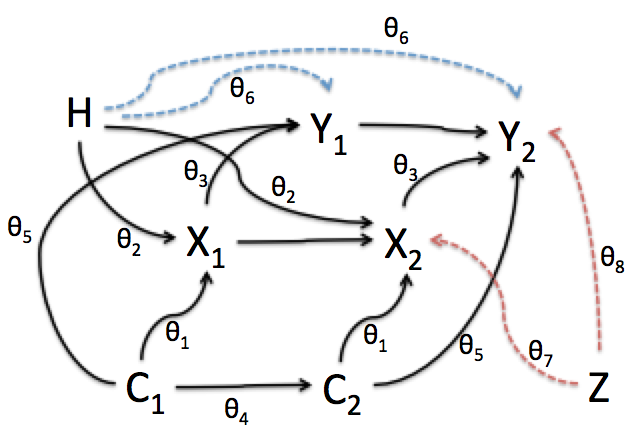
\includegraphics[width=12cm]{mypic2.png}
\caption{The two time-point model considered.  We do not suggest that this model will be adequate for all applications. However, it is sufficiently rich to provide a vehicle for investigating the consequences of preferential sampling, and for the application that is described in Section X of the paper.}
\centering
\end{figure}

\begin{figure}[h!]
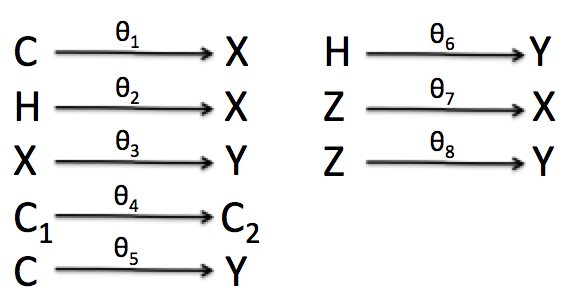
\includegraphics[width=9cm]{mypic1.png}
\caption{Parameters considered.}
\centering
\end{figure}


$\quad$

\begin{table}[h]
\begin{center}
 \begin{tabular}{||c | c c c c||} 
 \hline
  & & & \textbf{Representation} & \textbf{Interpretation} \\ [0.5ex] 
  \hline
 \textbf{Variable} & \textbf{if = 0} & \textbf{if $=$ 1}  &   & \\ 
 \hline\hline
 H & ealry & late &  Instrumental Variable & Calendar time  \\ 
 \hline
 C & ? & ? & Known Confounder  & ?\\ 
 \hline
 Y & ill & healthy & Outcome of interest  & Disease progression\\ 
 \hline
 Z & ? & ? & Unknown additional confounder &  \\ 
 \hline
X & no treatment  & treatment & Intervention of interest & Treatment \\ [0.5ex] 
 \hline\hline
  \textbf{Parameter} &   \textbf{if = 0} & \textbf{if $>$ 0}   & & \\ 
 \hline
 $\theta_{1}$  & \xmark & \xmark &\xmark  &\\ 
 \hline
 $\theta_{2}$    & \xmark & \xmark  & \xmark & \\ 
 \hline
 $\theta_{3}$   & Null is true & Alt. is true & intervention effect & treatment effect\\
 \hline
 $\theta_{4}$   & \xmark & \xmark & \xmark &\\
 \hline
 $\theta_{5}$   & \xmark & \xmark & \xmark &\\
 \hline
 $\theta_{6}$   & \xmark & \xmark & \xmark &\\
 \hline
 $\theta_{7}$   & \xmark & \xmark & \xmark &\\
 \hline
 $\theta_{8}$   & \xmark & \xmark & \xmark &\\
 \hline

\end{tabular}
\end{center}
\caption{Model Components.}
\end{table}






$\quad$


$\quad$

$\quad$

\newpage

Given an outcome measure, a treatment variable, a set of unmeasured confounders, and, possibly, a set of measured confounders, a variable satisfies the conditions of an instrumental variable (also referred to as an instrument) if the following conditions hold: 

\begin{itemize}
\item{(1) it is correlated with the treatment
variable}
\item{(2) given the treatment variable and all confounders (measured and unmeasured), it is conditionally independent of outcome; and}
\item{(3) it is independent of the entire set of unmeasured
confounders \cite{greenland2000introduction}.}
\end{itemize}


\textbf{With $Y_1$, without $H$:}

\begin{align*}
  Pr(Y_{2}=1 | do(X_{1}=x_{1}, X_{2}=x_{2})) & =  \sum_{y_{1}=0}^{1} \sum_{c_{1}=0}^{1} \sum_{c_{2}=0}^{1}
 Pr(C_{1}=c_{1}) \\
 &\cdot   Pr(C_{2}=c_{2} | C_{1}=c_{1}, X_{1}=x_{1}) \\
 & \cdot   Pr(Y_{1}=y_{1} | C_{1}=c_{1}, X_{1}=x_{1}) \\
 &\cdot   Pr(Y_{2}=1 | C_{2}=c_{2}, X_{2}=x_{2}, Y_{1}=y_{1})
\end{align*}

\textbf{With $Y_1$, and with $H$:}

\begin{align*}
  Pr(Y_{2}=1 | do(X_{1}=x_{1}, X_{2}=x_{2})) & =  \sum_{y_{1}=0}^{1} \sum_{c_{1}=0}^{1} \sum_{c_{2}=0}^{1} \sum_{h=0}^{1}
 Pr(H=h) \cdot Pr(C_{1}=c_{1} | H=h) \\
 &\cdot   Pr(C_{2}=c_{2} | C_{1}=c_{1}, X_{1}=x_{1}, H=h) \\
 & \cdot   Pr(Y_{1}=y_{1} | C_{1}=c_{1}, X_{1}=x_{1}, H=h) \\
 &\cdot   Pr(Y_{2}=1 | C_{2}=c_{2}, X_{2}=x_{2}, Y_{1}=y_{1}, H=h)
\end{align*}

\textbf{Without $Y_1$, without $H$:}

\begin{align*}
  Pr(Y_{2}=1 | do(X_{1}=x_{1}, X_{2}=x_{2})) & =  \sum_{c_{1}=0}^{1} \sum_{c_{2}=0}^{1}
 Pr(C_{1}=c_{1}) \\
 &\cdot   Pr(C_{2}=c_{2} | C_{1}=c_{1}, X_{1}=x_{1}) \\
 &\cdot   Pr(Y_{2}=1 | C_{2}=c_{2}, X_{2}=x_{2})
\end{align*}

\textbf{Without $Y_1$, with $H$:}

\begin{align*}
  Pr(Y_{2}=1 | do(X_{1}=x_{1}, X_{2}=x_{2})) & =  \sum_{c_{1}=0}^{1} \sum_{c_{2}=0}^{1} \sum_{h=0}^{1}
 Pr(H=h) \cdot Pr(C_{1}=c_{1} | H=h) \\
 &\cdot   Pr(C_{2}=c_{2} | C_{1}=c_{1}, X_{1}=x_{1}, H=h) \\
 &\cdot   Pr(Y_{2}=1 | C_{2}=c_{2}, X_{2}=x_{2}, H=h)
\end{align*}




 \section{Methods}
 
 
 \textbf{Frequentist g-comp with logistic model:}
$Pr(A=1 | B=b, C=c) = predict(logistic(Pr(A=1 | B=b, C=c)))$

$\quad$

\textbf{Bayesian g-comp with Uniform priors:}
$Pr(A=1 | B=b, C=c) \sim Beta(1+ \sum_{i=1}^{n}1_{(A=1,B=b,C=c)}(x_{i}), 1+ \sum_{i=1}^{n}1_{(A=0,B=b,C=c)(x_{i})})$

$\quad$

 
- run down of the simple sandbox of two time-points, everything binary 
	- g-computation (perhaps motivated several different ways)
	- IV idea

Comparison in a focussed scenario
-	confounding by indication present (C encourages treatment start)
-	different possible forms of treatment effect (through C and/or around C)
-	both sets of assumptions met

Comparison across a broad range of scenarios

-	set up distribution giving rise to a wide array of states of the world
-	look for patterns, e.g., is the power of the g-computation driven only by theta11-theta00, or are there other important factors
    
Violations of assumptions

-	any defensible sense of one procedure being more robust than the other
-	how quickly is power lost as we relax assumptions


\begin{figure}[h!]
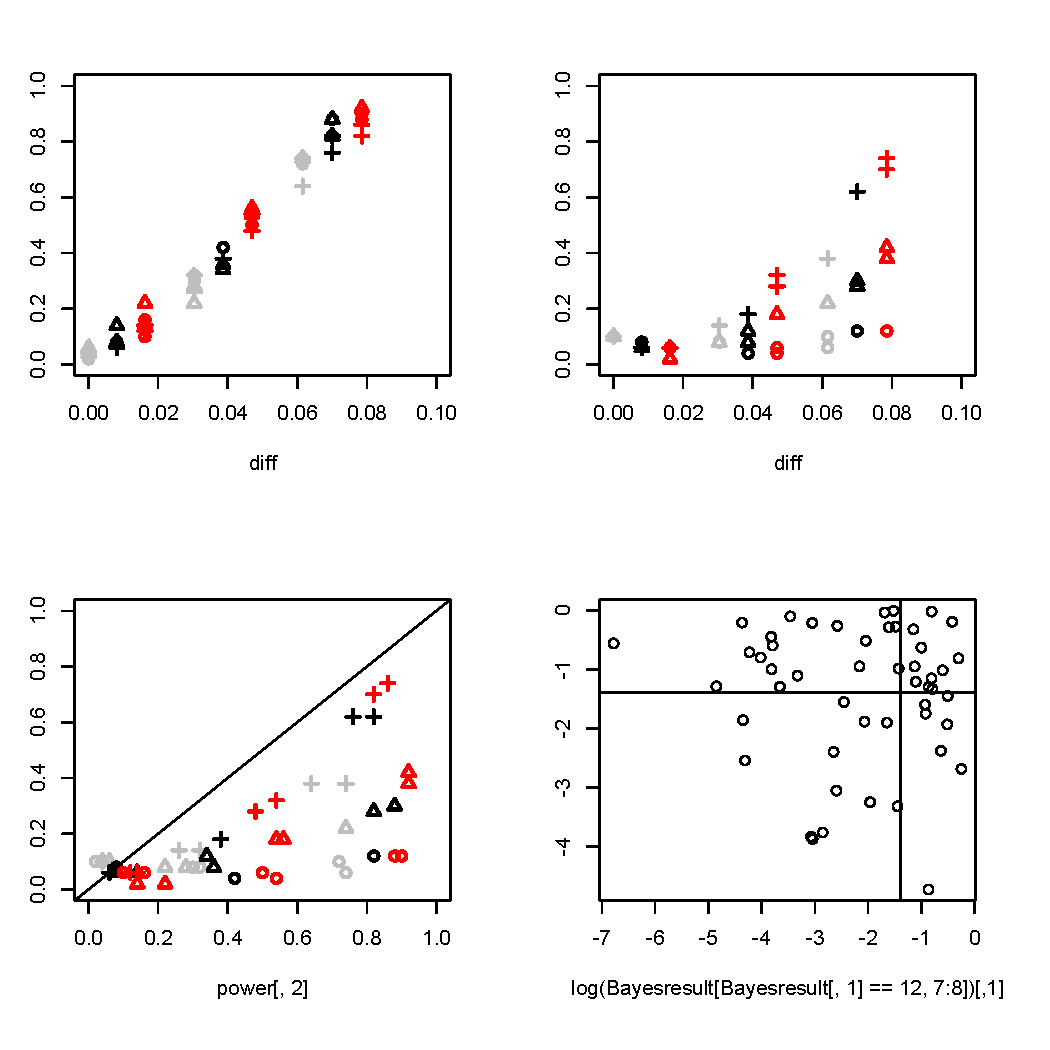
\includegraphics[width=12cm]{RplotPaul.pdf}
\caption{Results of Simulation study.}
\centering
\end{figure}



 \section{Application}

 \section{Discussion}
\newpage

\bibliography{gcomp_refs} 
\bibliographystyle{ieeetr}


\end{document}  